\documentclass[12pt, a4paper, openany]{book}
\usepackage[inline]{enumitem}
\usepackage{../generalStyle}

\graphicspath{ {./img/} }

\begin{document}

\title{Fisica}
\author{Fabio Ferrario}
\date{2022/2023}
\maketitle

\tableofcontents

\chapter{Introduzione}

\section{Il corso}
\subsection*{Turno 1}
Il corso di fisica (turno 1) verrà svolto da:
\begin{itemize}
    \item Davide Gerosa (Responsabile corso)
    \item Costantino Pacilio (Esercitatore)
\end{itemize}
\paragraph*{Orario} Per il turno 1, il corso coprirà 48 ore di lezione frontale e 20 ore di esercitazioni:
\begin{itemize}
    \item Lunedì 13.30-16.30 U3-08, Lezione.
    \item Martedì 14.30-16.30 U2-02, Esercitazione.
    \item Mercoledì, 8.30-10.30 U1-09, Lezione.
\end{itemize}
\subsection*{Turno 2}
Il turno 2 verrà erogato da:
\begin{itemize}
    \item Alberto Bravin (Lezioni)
    \item Mario Marini (Esercitazioni)
\end{itemize}
\begin{itemize}
    \item Lunedì 8.30-11.30 U9-01, Lezione.

\end{itemize}
Le esercitazioni saranno ogni 8 ore di lezione (2 ore esercitazione)

\paragraph*{testo di riferimento} \emph{D.Halliday, R. Resnick. Fondamenti di Fisica (vol. 1 e 2), Casa Editrice Ambrosiana}.

\section{Il Programma}
\paragraph*{Prerequisiti} Le nozioni acquisite nel corso di Analisi Matematica, fra cui derivate ed integrali.

\paragraph*{Contenuti Sintetici} del programma:
\begin{enumerate}
    \item Meccanica.
    \item Gravitazione.
    \item Fluidodinamica.
    \item Onde.
    \item Termodinamica.
    \item Elettromagnetismo.
\end{enumerate}

\paragraph*{Programma Esteso}

\begin{enumerate}
    \item \textbf{Meccanica}.
          \small{\begin{enumerate*}[label=(\roman*)]
                  \item Sistemi di coordinate e vettori.
                  \item Moto in una e più dimensioni.
                  \item Moto rettilineo uniforme, uniformemente accelerato, parabolico, armonico.
                  \item Leggi di Newton.
                  \item Energia cinetica, energia potenziale principio di conservazione.
                  \item Centro di massa.
                  \item Corpo rigido.
                  \item Momento lineare.
                  \item Moti di rotazione e di rotolamento.
                  \item Momento angolare, momento di inerzia, momento torcente.
                  \item Moti relativi.
              \end{enumerate*}}
    \item \textbf{Gravitazione}.
          \small{\begin{enumerate*}[label=(\roman*)]
                  \item Leggi di Keplero.
                  \item Legge di gravitazione universale.
                  \item Campo gravitazionale.
                  \item Legge di Gauss.
                  \item Velocità di fuga.
                  \item Potenziale efficace.
              \end{enumerate*}}
    \item \textbf{Fluidodinamica}.
          \small{\begin{enumerate*}[label=(\roman*)]
                  \item Fluidi, densità e pressione.
                  \item Legge di stevino.
                  \item Principio di Pascal.
                  \item Forza di Archimede.
                  \item Equazione di Continuità.
                  \item Equazione di Bernoulli.
              \end{enumerate*}}
    \item \textbf{Onde}.
          \small{\begin{enumerate*}[label=(\roman*)]
                  \item Oscillatore armonico.
                  \item Pendolo semplice.
                  \item Oscillatore smorzato.
                  \item Risonanza.
                  \item Concetto di onda.
                  \item Onda piana.
                  \item Periodo, lunghezza d'onda, velocità.
                  \item Riflessione e interferenza.
                  \item Onde stazionarie.
                  \item Onde sonore.
                  \item Battimenti.
                  \item Effetto Doppler
              \end{enumerate*}}
    \item \textbf{Termodinamica}.
          \small{\begin{enumerate*}[label=(\roman*)]
                  \item Temperatura e calore.
                  \item Calore specifico, calore latente.
                  \item Energia interna.
                  \item Primo principio della termodinamica.
                  \item Trasformazioni termodinamiche.
                  \item Trasmissione del calore (conduzione, convezione, irraggiamento).
                  \item Legge dei gas perfetti.
                  \item Teoria cinetica dei gas.
                  \item Irreversibilità, entropia.
                  \item Secondo principio della termodinamica.
                  \item Macchine termiche.
                  \item Ciclo di Carnot.
                  \item Zero assoluto.
              \end{enumerate*}}
    \item \textbf{Elettromagnetismo}.
          \small{\begin{enumerate*}[label=(\roman*)]
                  \item Carica elettrica.
                  \item Legge di Coulomb.
                  \item Campo elettrico.
                  \item Legge di Gauss.
                  \item Potenziale.
                  \item Conduttori.
                  \item Condensatori.
                  \item Corrente elettrica.
                  \item Legge di Ohm.
                  \item Legge delle maglie, legge dei nodi.
                  \item Circuito RC.
                  \item Campo magnetico.
                  \item Forza di Lorentz.
                  \item Legge di Biot-Savart.
                  \item Legge di Ampere.
                  \item Induzione elettromagnetica.
                  \item Legge di Faraday-Lenz.
                  \item Circuito RL.
                  \item Oscillazione LC.
                  \item Oscillazione Smorzata RLC.
                  \item Cenni di magnetismo nei materiali.
                  \item Legge di Ampere-Maxwell.
                  \item Correnti di spostamento.
                  \item Equazioni di Maxwell.
                  \item Onde elettromagnetiche.
                  \item Velocità della luce.
              \end{enumerate*}}
\end{enumerate}

\section{Esame}
L'esame ha \emph{una prova scritta e una orale facoltativa}.
\paragraph*{Prova scritta}
La prova scritta consite in alcuni esercizi da svolgere e alcune domante teoriche.
Ha una durata di 2 ore, il voto massimo è 30/30 e \emph{non vengono sottratti punti per le risposte sbagliate}.
Ogni esercizio ha l'indicazione del punteggio e le risposte devono essere complete.
è consentito l'utilizzo della calcolatrice (non grafica) ma \emph{non del formulario}.
\paragraph*{Prova orale}
Totalmente facoltativa, ha un punteggio di $\pm 5$ ed è necessaria per il raggiungimento della \emph{lode}.

\chapter{Materiale Propedeutico}
\section{Trigonometria}
\subsection*{Angoli e la loro Misura}
Quando vogliamo misurare un angolo possiamo usare due misure: \emph{Gradi} e \emph{Radianti}.
\definizione{
    \textbf{L'angolo di un grado} è \emph{la trecentosessantesima parte di un angolo giro}.
    La misura in gradi dell'angolo giro è 360°
    \\\textbf{L'angolo di un radiante} è quell'angolo che su una circonferenza (di centro nell'origine dell'angolo)
    intercetta un angolo di lunghezza pari al raggio. La misura in radianti dell'angolo giro è $2\pi$.
    \\\emph{Più in generale}, la misura $\alpha$ in radianti di un angolo al centro è il rapporto
    \[\alpha = \frac{l}{r}\]
    Dove $l$ è la misura dell'arco sotteso dall'angolo al centro e $r$ è il raggio della circonferenza.
}
\paragraph*{La trasformazione delle misure}
\definizione{
    Se $\alpha$ è la misura in radianti di un angolo e $z°$ la sua misura in gradi, si ha:
    \[\alpha : z° = \pi : 180°\]
}
In parole povere:
\begin{itemize}
    \item $rad \to deg$: $(\alpha \cdot 180)/\pi$
    \item $deg \to rad$: $(z$°$ \cdot \pi)/180$
\end{itemize}

\subsection*{Seno, Coseno e Tangente}
\definizione{
    Sia P un punto appartenente alla circonferenza C di centro (0,0) e di raggio 1 (circonferenza trigonometrica),
    e sia $\alpha$ l'angolo positivo descritto dal semiasse positivo delle ascisse per sovrapporsi alla semiretta $OP$.
    \\Allora il punto $P$ ha coordinate:
    \[P=(\cos\alpha,\sin\alpha)\]
}
\paragraph*{Periodicità}
Poichè la circonferenza C è lunga $2\pi$, sommando $2\pi$ a $\alpha$ si fa compiere a $P$
un giro completo e si giunge allo stesso punto P. 
\\Quindi, per ogni $\alpha$,
\[\sin(\alpha) = \sin(\alpha + 2\pi) \wedge \cos(\alpha) = \cos(\alpha+2\pi)\]
Si dice che le funzioni seno e coseno sono periodiche con periodo $2\pi$
%Mettere la definizione di Tangente

\subsection*{Teoremi trigonometrici sul triangolo rettangolo}
Se abbiamo un vettore (di cui sappiamo il modulo) e un angolo su un asse cartesiano possiamo dividere il vettore sugli assi usando i
\emph{teoremi trigonometrici sul triangolo rettangolo}.
\\Se disegnamo un angolo rettangolo che usa come ipotenusa il nostro vettore, usiamo la definizione per trovare i due cateti:
\definizione{
    La misura di un \emph{cateto} è uguale a quella dell'ipotenusa per il seno dell'angolo opposto, oppure per il coseno dell'angolo adiacente.
    \\La misura di un cateto è uguale a quella dell'altro cateto per la tangente dell'angolo opposto.
}

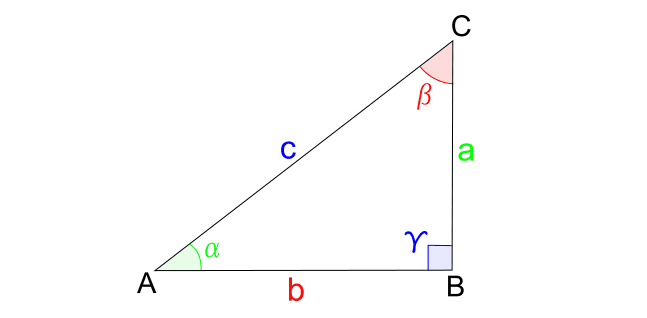
\includegraphics[width=\textwidth]{triangoloRettangolo.png}
Quindi, prendendo in considerazione l'immagine:
\\Per il cateto $a$:
\begin{itemize} %controllare n'attimo la terminologia
    \item  $\beta$ è l'angolo \emph{adiacente all'ipotenusa}
    \item  $\alpha$ è l'angolo \emph{opposto all' ipotenusa}
\end{itemize}
Di conseguenza, avendo l'ipotenusa $c$ e gli angoli $\alpha$ e $\beta$, il cateto $a$ equivale a:
\[ a = c\cdot \cos(\beta) \vee a = c\cdot \sin(\alpha) \]
quindi: \textbf{cateto = ipotenusa $\cdot$ seno(opposto)} oppure \textbf{cateto = ipotenusa $\cdot$ coseno(adiacente)}
\chapter{Introduzione alla Fisica}

\subsection{Introduzione alla Fisica}
La fisica studia i fenomeni naturali e le leggi che li governano.
Si basa sulla \emph{Semplificazione} dei concetti, tramite \emph{Modelli e Approssimazioni}.


\paragraph{Antica $\neq$ Moderna} In antichità la fisica era legata alla filosofia e alla religione
e vigeva il principio di autorità, \emph{"ipse dixit"} (Aristotele).
\\La fisica moderna invece nasce con Galileo, separando ciò che è oggettivo da ciò che è soggettivo.
Si basa sulle cose \textbf{Misurabili}.
\paragraph{Il metodo scientifico} è un sistema che permette a chiunque abbia i mezzi di ripetere un esperimento.
La scienza non è una religione, vale infatti il principio di Falsicabilità:
\begin{center}
    \emph{Principio di Falsicabilità}: Se un esperimento da risultati contrastanti alle teorie correnti, allora c'è bisogno di una nuova teoria.
    \\Ovvero ogni teoria è valida finchè non ne esiste una migliore.
\end{center}
\section{Le unità di misura}
Il Sistema Internazionale definisce varie unità di misure standard: lunghezza, massa, mole, etc\dots
\\In una formula, le dimensioni devono essere \underline{Bilanciate}.
\subsection{Le cifre significative}
Un concetto molto importante è quello delle cifre significative.
\\Ogni Misurazione è affetto da \textbf{incertezze}:
\begin{enumerate}
    \item Indeterminazioni nell'effettuare la Misurazione
    \item Limite di sensibilità dello strumento usato
    \item Capacità dello sperimentatore
    \item \emph{Aleatorietà} della sperimentazione
\end{enumerate}
L'incertezza può essere \emph{determinata} oppure \emph{stimata}, in base al caso in esame.
\paragraph{Contare gli 0} Quando facciamo una misurazione, il numero di cifre significative è sempre importante, anche quando si tratta di 0,
infatti vale che $39,0 \neq 39,00$ \emph{Perchè} 3 cifre significative $\neq$ 4 cifre significative.
\paragraph{Proprietà delle cifre significative}
\begin{itemize}
    \item \textbf{Moltiplicando (o dividendo)} quantità affette da incertezza, il numero determinato ha \emph{lo stesso numero di cifre significative della Meno accurata delle quantità}
    \item \textbf{Sommando (o sottraendo)} Vale la stessa proprietà.
\end{itemize}



\paragraph{Ordini di grandezza}
è un'approssimazione di un numero e indica la potenza di 10 più vicina al numero dato

\subsection{Vettori e scalari} Esistono due tipi di grandezze nella fisica:
\begin{itemize}
    \item \textbf{Grandezze Scalari}: determinate da un solo numero (la misura) ed una unità di misura.
    \item \textbf{Grandezze Vettoriali}: determinate da più valori $\to$ \emph{Modulo (grandezza), direzione e verso}
          \begin{itemize}
              \item Quando diventa necessario conoscere un punto specifico di localizzazione del vettore (l'origine) si usa la dizione Vettore Applicato.
          \end{itemize}
\end{itemize}
\paragraph{I Vettori e le proprietà}
%I vettori vengono indicati in grassetto o con freccia sormontata: \textbf{a,AB}, \overrightarrow{AB} o \overrightarrow{v}, con il modulo generalmente scritto in corsivo \emph{v}, oppure AB o $|$\overrightarrow{AB}$|$

\subparagraph*{Algebra Vettoriale}

\begin{itemize}
    \item a=b : vettori uguali \emph{sse} hanno lo stesso modulo, direzione e verso.
    \item b=-a: vettori opposti \emph{sse} hanno stesso modulo e direzione ma verso opposto
    \item vettore nullo: sse ha modulo nullo
\end{itemize}
Somma e differenza di vettori:

\chapter{Cinematica di un Punto 1D}
\paragraph{introduzione}
Sia dato un sistema di riferimento orientato x.
Sia dato un punto materiale.
Avremo queste tre formule (dei \emph{moduli}):
\begin{itemize}
    \item \textbf{Spostamento}: $s=\Delta x = x_2-x_1$
    \item \textbf{Velocità Media}: $v_m = \frac{(x_f-x_i)}{(t_f-ti)} = \frac{\Delta x}{\Delta t}$
    \item \textbf{Velocità Istantanea}: $v_x = \lim_{t\to 0} \frac{\Delta x}{\Delta t} = \frac{dx}{dt}$
\end{itemize}
\paragraph{Spostamento $\neq$ Distanza}
Lo \emph{spostamento} è un vettore che si annulla quando il punto torna alla posizione di partenza (in un tempo diverso),
mentre la distanza è uno scalare che indica \emph{tutta la distanza che il punto ha già percorso}.
\paragraph{L'accelerazione} L'acelerazione è la variazione della velocità nel tempo.
Le formule dell'acelerazione sono:
\begin{itemize}
    \item \textbf{Accelerazione Media}: $a_m = \frac{v_f-v_i}{t_f-t_i} = \frac{\Delta v}{\Delta t}$
    \item \textbf{Accelerazione Istantanea}: $a_x = \lim_{\Delta t \to 0} = \frac{\Delta v}{\Delta t} = \frac{dv_x(t)}{dt}= \frac{d}{dt}\frac{dx}{dt} = \frac{d^2x}{dt^2}$
\end{itemize}
\emph{L'accelerazione è la derivata della velocità}.
\subsection{I tipi di Moto}
Esistono tre tipi di moto del punto materiale 1D, ed essi variano in base all'accelerazione e alla velocità:
\paragraph*{Moto Vario} Se l'accelerazione varia continuamente, il moto non è facile da analizzare. Infatti non lo vedremo in questo corso.
\paragraph*{Moto rettilineo uniforme}\emph{Velocità costante, accelerazione: 0}.
\\Questo tiop di moto si verifica quando la velocità è costante e ha le seguenti formule per velocità istantanea e spostamento:
\begin{itemize}
    \item $x(t)= x_i + v_x \cdot t$
    \item $v_x = k$, con $k\in R$ quindi COSTANTE.
\end{itemize}
\paragraph*{Moto Uniformemente accelerato} \emph{Con accelerazione costante}.
\\In questo caso l'accelerazione istantanea = accelerazione media in ogni istante, e la velocità cambia \emph{linearmente} durante il moto.
\begin{itemize}
    \item $x(t) = x_i + v_x\cdot t +\frac{1}{2} a_x \cdot t^2$
    \item $v_x(t) = v_{ix} + a_x \cdot t$
    \item $a_x = k1$ con $k1 \in R$.
\end{itemize}
Notare che se $a_x=0$ si ottiene il moto rettilineo uniforme.

\paragraph*{La Caduta di un Grave}
Un caso particolare del moto rettilineo uniforme è la caduta di un grave, in cui la velocità iniziale è \emph{zero} e
l'accelerazione è quella di gravità, ovvero $g\approx 9,81m/s^2$ ed è $\pm$ costante in tutto il mondo.
Essendo il grave in caduta l'accelerazione è negativa, quindi usando le formule del moto uniformemente accelerato e applicando $a=-g=-9,81m/s^2$ otteniamo:
\begin{center} %box formule da inserire
    $y(t)=-\frac{1}{2} g\cdot t^2$\\$ v(t) = -g \cdot t$
\end{center}
Se esplicitiamo la fromula rispetto a t (per sapere quanto ci mette a cadere un grave) e indichiamo con h l'altezza da cui cade otteniamo:
$$t_c =\sqrt{\frac{2h}{g}}$$
Nota che la massa di un oggetto è irrilevante, quindi (nel vuoto) ci mettono tutti lo stesso tempo ad arrivare a terra.

\paragraph*{le equazioni Cinematiche}
Siccome la \emph{Derivazione è la funzione inversa dell'integrazione e viceversa} e l'accelerazione è la derivata della velocità che è la derivata dello spostamento
possiamo da una ottenere l'altra e viceversa:
\begin{itemize} %\to da sostituire con \implies o la doppia implicazione
    \item $a_x = \frac{dv_x}{dt} \to dv_x = a_xdt \to v_x = \int a_x dt + C$
          \begin{itemize}
              \item se $a_x$ è costante allora $v_x = ... = a_x t + C$ (con C velocità iniziale)
          \end{itemize}
    \item $v_x = \frac{dx}{dt} \to dx = v_xdt \to x = \int v_xdt + C$
          \begin{itemize}
              \item se la velocità non è costante allora $v_x(t) = v_i + a_x \cdot t$
          \end{itemize}
\end{itemize}
\section*{La cinematica nel punto materiale 2D}
Fin'ora abbiamo considerato solo il moto in una dimensione, adesso considereremo quella in 2 dimensioni.
Quando studio il movimento 2D posso studiarlo in due modi: o studio il suo movimento in un piano o studio il cambiamento delle sue coordinate nel tempo.
\subparagraph*{Movimento in un piano} Per studiare il movimento nel piano (quindi senza usare le coordinate) posso considerare ogni
punto come un vettore $r$ avente punto di applicazione in 0.
%immagine lez2slide11
In questo caso posso considerare lo spostamento da A a B nel tempo $\Delta t = t_f-t_i$ come $\Delta r = r_f-r_i$

\paragraph*{Estensione del caso 1D} Le stesse formule monodimenisonali valgono anche per il moto bidimensionale, bisogna solo usare i vettori.
\\Per estensione del caso 1D quindi la velocità media sarà:
\begin{center}
    $\overline{v} = \frac{\Delta r}{\Delta t}$ poichè t è uno scalare, $\overline{v}$ ha la stessa direzione e verso di $\Delta r$
\end{center}
Analogamente la velocità istantanea sarà
\begin{center}
    $v = lim_{\Delta \to 0 } \frac{\Delta r}{\Delta t} = \frac{dr}{dt}$
\end{center}
Il vettore velocità è quindi la derivata del vettore posizione rispetto al tempo e in un punto avrà direzione della tangente
alla curva dello spostamento in quel punto.
\\Quando un punto materiale viaggia su una traiettoria curva in 2D, il vettore velocità \emph{varia di direzione punto per punto anche se il modulo rimane costante} e si verifica quindi una \textbf{accelerazione}.
\\L'accelerazione media si calcola:
\[\overline{a}=\frac{v_f-v_i}{t_f-t_i}= \frac{\Delta v}{\Delta t}\]
Analogamente ai casi simili già visti, $a_m$ avrà la stessa direzione del vettore $\Delta v$
%inserire accelerazione istantanea lez2slide13
\paragraph*{riassumento}L'accelerazione di una particella in moto in uno spazio 2d può dunque corrispondere à:
\begin{enumerate}
    \item una variazione del modulo di v
    \item una variazione di direzione a modulo costante di v
    \item una combinazione delle due
\end{enumerate}
Un utile notazione diversa degli stessi concetti la si ha considerando le componenti cartesiane, in cui l'accelerazione è la somma delle acc di tutte le dimensioni cartesiane.
$$ a = \frac{dv_x}{dt}i + \frac{dv_y}{dt}j + \frac{dv_z}{dt}k $$
\subsection*{Moto uniformemente accelerato in 2D}
Per detereminare le equazioni del moto in 2D si estendono i concetti per il moto 1D.
Questo passaggio logico è molto semplice: si \emph{scompone il moto 2D in 2 moti 1D} sugli assi XY.
\paragraph*{Moto con accelerazione costante}
%Adattando il caso 1D, quindi dividendo i moti 2D in due moti 1D, si ottiene che:
%\\$v_f = v_i + at \implies v_f = (v_{xi}i + v_{yj}j) + (a_xi + a_yj)t$ nelle sue componenti cartesiane.
Un moto 2D ad accelerazione costante è la \emph{composizione dei due moti indipendenti lungo x ed y}, di accelerazione costante rispettivamente $a_x$ e $a_y$:
% Formula
$$ v_f = v_i + at \implies \begin{cases}
        v_{xf} = v_{xi} +a_xt \\
        v_{yf} = v_{yi} +a_yt
    \end{cases}
$$
$$ r_f = r_i + v_it + \frac{1}{2}at^2 \implies \begin{cases}
        x_f = x_i + v_{xi}t + \frac{1}{2}a_xt^2 \\
        y_f = x_i + v_{yi}t + \frac{1}{2}a_yt^2
    \end{cases}$$
Nota che in alcuni casi le accelerazioni saranno nulle (moto costante) e le equazioni si semplificheranno.

\section{Il moto di un proiettile}
Il moto di un proiettile è di "facile" determinazione sotto due condizioni:
\begin{itemize}
    \item L'accelerazione di gravità è \emph{costante} lungo tutto il percorso del proiettile.
    \item La resistenza dell'aria è trascurabile.
\end{itemize}
Sotto queste condizioni il moto di un proiettile ha un'accelerazione costante ed è dunque di tipo parabolico.

\subsection{I calcoli}
Si consideri un proiettile lanciato con un vettore velocità iniziale $\overrightarrow{v_i}$ che forma un angolo $\theta_i$ con l'asse delle $x$:
\begin{center}
    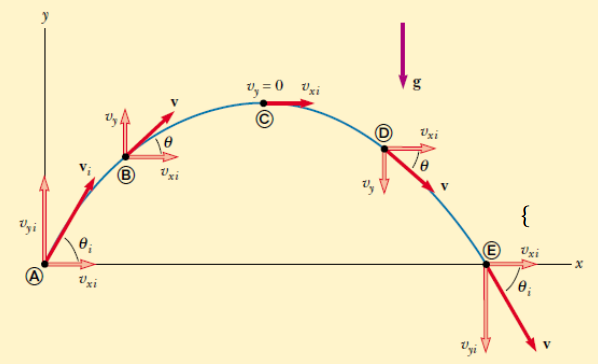
\includegraphics[width=\textwidth]{lez2slide19.png}
\end{center}
Si può notare che:
\begin{itemize}
    \item $a_x=0$: L'accelerazione $x$ (orizzontale) è zero
    \item $a_y= -g$: l'accelerazione $y$ è la forza di gravità verso il basso.
    \item $v_{xi} = v_i \cdot \cos \theta_i$: la velocità iniziale orizzontale è calcolata con il coseno dell'angolo.
    \item $v_{yi} = v_i \cdot \sin \theta_i$: analogamente la velocità verticale è calcolata con il seno.
    \item $x_i=y_i=0$ per la scelta dell'origine delle cooridnate.
\end{itemize}
Riassumendo, l'unica forza che agisce sul proiettile è quella di gravità ed agisce come accelerazione sulla componente verticale.

\paragraph*{Troviamo velocità e posizione finale}
Avendo questi dati ed utilizzando le formule per il moto in 2D si ottiene:
\begin{itemize}
    \item $v_xf = v_xi$ poichè non c'è alcuna accelerazione.
    \item $v_{yf} = v_{yi} - gt$, dato che la gravità rallenta il proiettile
\end{itemize}
\begin{itemize}
    \item $x_f = v_{xi}t = (v_i \cos \theta_i) t$ sostituendo con il calcolo della velocità in $x$.
    \item $y_f = v_{yi}t + \frac{1}{2} a_yt^2 = (v_i \sin \theta_i)t - \frac{1}{2} gt^2$ analogamente
\end{itemize}
Se risolviamo $x_f$ rispetto a $t$ e la inseriamo in $y_f$ otteniamo:
\[
    \begin{cases}
        x = (v_i \cos \theta_i) t \to t = \frac{x}{(v_i \cos \theta_i)} \\
        y = (tan \theta_i) x- (\frac{g}{2v_i^2\cos^2 \theta_i})x^2
    \end{cases}
\]
Si noti che $y=...$ è l'equazione di una parabola per l'origine degli assi.


\section*{Il moto circolare uniforme}
Il MCU è il moto di un punto materiale lungo una circonferenza, con modulo della veloctià costante.
Un'altra possibile definizione è la seguente: \emph{Dato un punto P sulla circonferenza, questo punto percorrerà spazi uguali in eguali intervalli di tempo.}
\paragraph*{L'accelerazione }Il modulo della velocità è costante, ma siccome c'è una variazione della direzione del vettore velocità $\implies$ c'è in gioco una acelerazione
(infatti è definita acelerazione la variazione nel tempo del vettore velocità).
\\Prendiamo in considerazione questo:
\begin{itemize}
    \item Consideriamo una circonferenza di raggio $r$.
    \item il punto materiale si muove a velocità di modulo costante lungo la traiettoria circolare.
    \item il vettore velocità è tangente alla traiettorie circolare.
    \item la variazione del vettore velocità $\Delta v$ nel limite di $\Delta t$ sempre più piccoli ha una direzione sempre più rivolta al centro della circonferenza.
\end{itemize}
\textbf{L'acelerazione istantanea} è diretta al centro della circonferenza, e per questo motivo si chiama acelerazione \textbf{centripeta}.
Il suo modulo è: $a_r = \frac{v^2}{r}$ (il pedice r indice che è diretta lungo il raggio r) con r raggio del cerchio.
\\Si chiama velocità tangenziale la velocità diretta lungo la circonferenza.
\\DEFINIZIONE: In un moto circolare uniforme l'accelerazione è diretta verso il centro del cerchio ed ha un modulo pari a $v^2/4$ dove v è il modulo della velocità tangenziale (costante) e r è il raggio del cerchio

\chapter{Le Forze}
Fin'ora abbiamo solo considerato le equazioni della cinematica, cioè il moto di particelle indipendenetemente dalle cause stesse del moto.
Per determinare le cause di un moto dovremmo considerare si ala massa del corpo, che le forze che agiuscono su questa massa.

In alcuni casi le Forze determinano degli \emph{spostamenti}, ovvero un moto, ma in altri casi applicando delle forze non si verificano moti, per esempio il fatto che stiamo seduti senza cadere al suolo.
\definizione{
    Un oggetto che stia fermo, o sia in moto rettilineo uniforme, accelera se e solo se
    la forza totale, come somma vettoriale delle forze,
    detta anche la \textbf{risultante delle forze}, è diversa da zero
}

\section{Newton}
Newton disse che "le forze determinano i cambiamenti di velocità delle masse", cioè delle \emph{Accelerazioni}.
\subsection{Principio di Inerzia - I Legge di Newton}
\paragraph*{Introduzione}
Si consideri un oggetto fermo su un piano, se lo si spinge orizzontalmente, si muoverà solo quando \emph{la forza applicata supererà la forza di attrito del tavolo}.

Per mantenere il corpo a velocità costante, bisognerà applicare una forza che eguagli la forza di attrito con il piano.
La forza di attrito quindi è una forza che va nella \textbf{direzione opposta} alla forza che stiamo applicando.
Se applichi una forza maggiore, l'oggetto accellererà.

\paragraph*{La legge}
La prima legge di Newton enuncia:
\definizione{
    Quando un punto materiale non è soggetto a forze esterne, oppure la loro risultante è nulla, allora il punto materiale ha una velocità \textbf{Costante o Nulla}.
}
\end{document}